\documentclass[11pt]{article}
\usepackage[T1]{fontenc}
\usepackage[utf8]{inputenc}
\usepackage{amsmath,amssymb}
\usepackage{booktabs}
\usepackage{tabularx}
\usepackage{xcolor}
\usepackage[most]{tcolorbox}
\usepackage{listings}
\usetikzlibrary{arrows.meta,positioning,shapes.misc}
\usepackage[margin=0.95in]{geometry}
\usepackage{hyperref}
\hypersetup{colorlinks=true,linkcolor=blue!50!black,urlcolor=blue!50!black}

\definecolor{askblue}{HTML}{1976D2}
\definecolor{amber}{HTML}{FFA000}
\definecolor{trapred}{HTML}{D32F2F}
\definecolor{chipgreen}{HTML}{2E7D32}

\newtcolorbox{idea}[1][]{breakable,colback=askblue!6!white,colframe=askblue,fonttitle=\bfseries,title={#1}}
\newtcolorbox{recall}[1][]{breakable,colback=amber!8!white,colframe=amber,fonttitle=\bfseries,title={#1}}
\newtcolorbox{trap}[1][]{breakable,colback=trapred!6!white,colframe=trapred,fonttitle=\bfseries,title={#1}}
\newtcolorbox{good}[1][]{breakable,colback=chipgreen!6!white,colframe=chipgreen,fonttitle=\bfseries,title={#1}}

\lstset{basicstyle=\ttfamily\small,columns=fullflexible,keepspaces=true,frame=single,
        framerule=0.3pt,rulecolor=\color{gray!60},xleftmargin=4pt,breaklines=true}

\setlength{\parindent}{0pt}
\setlength{\parskip}{5pt}
\newcommand{\lam}{\lambda}

\title{\textbf{rounderr}\\[2pt]\large an AI powered reverse mode rounding error interpreter in Python\\[2pt]\normalsize design guide, Part I the engine, Part II the AI layer, Part III one machine and Bean}
\author{Eric Shi \quad CS 4999 with Dr.\ David Bindel}
\date{November 2026}

\begin{document}
\maketitle

\begin{idea}[What the program does in one breath]
You type a formula (plain text, LaTeX, or a line by line tape). The program reads it back to you the way it understood it, asks for the numbers, runs the formula once forward while writing a tape, runs the tape once backward to get every line's weight $\lam_i$, and then prints three kinds of numbers. \textbf{What actually happened} (computed value, 60 digit true value, actual error, and the first order prediction of that error from the measured slips). \textbf{What the error might be} (the worst case ceiling, the typical size, the problem's condition number $\kappa$, the algorithm's amplification $A$, and Bindel's backward error $\beta$). \textbf{Why and what to do} (which line carries the blame, which subtraction magnifies it, and rewrite candidates you can pick and rerun with the same numbers). Everything can be written out as a LaTeX report.
\end{idea}

\section*{Part I \quad The engine (\texttt{rounderr.py})}
\section{The math it runs}

The notation is the one from the whiteboard and from Bindel's FPTalks 2026 slides. The content is Linnainmaa's 1970 thesis and 1976 paper.

\begin{recall}[Tape, slips, adjoint, three readings of one equation]
\textbf{Tape.} Every rounded step is one line $t_i = G_i(t_{<i}, x)$. Written as a system,
\[
F(t,x) = t - G(t,x) = 0, \qquad y = w^{T} t, \quad w = e_n \text{ picks the last line}.
\]
\textbf{Slips.} The machine does not compute $t_i$ but $\hat t_i$. The slip of line $i$ is the computed value minus the exact operation applied to the already rounded operands,
\[
\rho_i = \hat t_i - G_i(\hat t, \hat x), \qquad |\rho_i| \le d_i\,|t_i|\,u ,
\]
which is Linnainmaa's local error $r_i$ (his equation 3). $u = 2^{-53}$ for double. $d_i = 1$ for an IEEE operation, $2$ for a library function (1 ulp), $0$ for a step that is exact.

\textbf{Linearize} $F(\hat t,\hat x) = \rho$ around the exact run,
\[
F_t\,\Delta t + F_x\,\Delta x = \rho, \qquad \Delta y = w^{T}\Delta t
\quad\Longrightarrow\quad
\Delta y = \lam^{T}\rho - \lam^{T}F_x\,\Delta x, \qquad \lam = F_t^{-T} w .
\]
$F_t = I - G_t$ is unit lower triangular, so $F_t^{T}\lam = w$ is a back substitution. That back substitution \emph{is} the reverse sweep (Linnainmaa's Algorithm T).

\textbf{Three readings.}
\begin{center}
\begin{tabular}{@{}lll@{}}
\toprule
set & result & name \\
\midrule
$\rho = 0$ & $\nabla_x y = -F_x^{T}\lam = G_x^{T}\lam$ & reverse mode gradient \\
$\Delta x = 0$ & $\Delta y = \lam^{T}\rho$ & forward error (Linnainmaa, first order) \\
$\Delta y = 0$ & $\lam^{T}F_x\,\Delta x = \lam^{T}\rho$, \ $\|\Delta x\|_2 = |\lam^{T}\rho| / \|g\|_2$ & backward error, $g = \nabla_x y$ \\
\bottomrule
\end{tabular}
\end{center}

\textbf{Numbers the program prints.} With $v_i = \lam_i d_i t_i$ over the tape lines,
\[
\text{ceiling} = u\sum_i |v_i|,\qquad
\text{typical} = \tfrac{u}{\sqrt 3}\,\|v\|_2,\qquad
\text{predicted} = \sum_i \lam_i \rho_i \ \ (\text{measured } \rho_i),
\]
\[
\kappa = \frac{\sum_j |g_j x_j|}{|y|},\qquad
A = \frac{\sum_i |v_i|}{|y|},\qquad
\beta_1 = \frac{\|v\|_1}{\|g\|_2\,\|x\|_2},\qquad
\beta_2 = \frac{\|v\|_2}{\|g\|_2\,\|x\|_2}.
\]
$\kappa u$ is the relative error the \emph{problem} forces on any algorithm. $A u$ is what \emph{this algorithm} allows. The verdict rule is $A \le \max(10, n)\max(1,\kappa)$ means stable, otherwise unstable, where $n$ is the number of rounded steps (the allowance grows with $n$, as the $n\varepsilon$ bounds Bean proves for sums and Horner do). $\beta_1$ is the smallest relative input change (in units of $u$) that would explain the worst case output error. Small $\beta$ means backward stable.
\end{recall}

\begin{good}[Worked numbers, the quadratic root $y = -b + \sqrt{b^2 - c}$ at $b = 1000$, $c = 1$]
\begin{center}
\begin{tabular}{@{}llrrrl@{}}
\toprule
line & & $t_i$ & $d_i$ & $\lam_i$ & note \\
\midrule
$t_2 = -b$ & & $-1000$ & 0 & 1 & sign only \\
$t_3 = b\cdot b$ & & $10^{6}$ & 0 & $5\times10^{-4}$ & small integers, exact \\
$t_4 = t_3 - c$ & & $999999$ & 0 & $5\times10^{-4}$ & small integers, exact \\
$t_5 = \sqrt{t_4}$ & & $999.9995$ & 1 & 1 & the only slip \\
$t_6 = t_2 + t_5$ & & $-5.0000013\times10^{-4}$ & 0 & 1 & Sterbenz, exact \\
\bottomrule
\end{tabular}
\end{center}
Gradient $(\partial y/\partial b,\ \partial y/\partial c) = (5\times10^{-7},\ -5\times10^{-4})$, so $\kappa = 2$. Ceiling $= u\cdot 999.9995 = 1.1\times10^{-13}$, which is $A = 2\times10^{6}$ in units of $u$ (charging every line once gives the September number $2000\,u$ absolute, $4\times10^{6}\,u$ relative). Actual error $-4.36\times10^{-14} = -7.9\times10^{5}u$, and $\sum\lam_i\rho_i$ predicts exactly that. $\beta_1 = 2000$. Verdict unstable, $A/\kappa = 10^{6}$. The program finds the rewrite $-c/(b+\sqrt{b^2-c})$ by itself. Rerun with the same numbers it has $A = 2.5$ and actual error $-0.05\,u$.
\end{good}

\section{How it is built, step by step}

The file is one Python module, \texttt{rounderr.py}, about 1000 lines in nine numbered sections. Each step below names the section and says what to write.

\subsection*{Step 1 \quad Read the formula (section 1, the reader)}
\begin{enumerate}
\item \textbf{Normalize.} Replace unicode ($\times$, $\div$, $\surd$, $\pi$, $^2$). If a backslash is present, expand LaTeX with a tiny scanner. \verb|\frac{A}{B}| becomes \verb|((A)/(B))| (recursive, so nesting works), \verb|\sqrt{A}| becomes \verb|sqrt(A)|, \verb|\sin| becomes \verb|sin|, \verb|\left| and \verb|\right| are dropped. Then \verb|^| becomes \verb|**|, braces become parentheses, \verb/|x|/ becomes \verb|abs(x)|.
\item \textbf{Tokenize with Python's own tokenizer.} No hand written parser. Walk the tokens and insert \verb|*| between a value and a value (\verb|2x|, \verb|4ac|, \verb|(a)(b)|, \verb|sin(x)cos(x)|). A multi letter name that is not a known function, not declared, and not of the form letter plus digits is split into letters (\verb|ac| becomes \verb|a*c|). \verb|sin x| becomes \verb|sin(x)|. \verb|ln| becomes \verb|log|. Every guess is pushed to a \texttt{notes} list.
\item \textbf{Tidy and echo.} \verb|ast.parse| then \verb|ast.unparse| gives a clean string. Print ``I read it as'' plus the notes, and ask for confirmation. Variables are the names that are never assigned, in order of first use.
\item \textbf{Scripts.} Lines with \verb|=| are a tape you wrote by hand. Each left side becomes a name the later lines can use. The last line is the output.
\end{enumerate}

\begin{trap}[Why not sympy for the reading]
\texttt{sympy.parse\_expr} rewrites $a/b$ as $a\cdot b^{-1}$ and reorders sums. That changes the tape, so it changes the rounding analysis. The \texttt{ast} module keeps the user's exact order and keeps subtraction and division as what they are. That is also why there is no \texttt{eval} anywhere.
\end{trap}

\subsection*{Step 2 \quad Build the tape (section 2)}
A \texttt{Line} holds \texttt{op}, the indices of its operands, and later its value, slip, $d$, partials and $\lam$. Walk the AST once with a recursive \texttt{build(node)} that returns the index of the line it made.
\begin{center}
\begin{tabular}{@{}ll@{}}
\toprule
AST node & tape line \\
\midrule
\texttt{Constant 0.1} & \texttt{const} line (storing $0.1$ already rounds, so it is a line) \\
\texttt{Name b} & the input line made at the start \\
\texttt{BinOp +, -, *, /} & \texttt{add sub mul div} with two operand indices \\
\texttt{x ** 2} & \texttt{sq}, one multiply, one rounding \\
\texttt{x ** 3} up to \texttt{** 8} & a chain of multiplies, as a numerical program would write it \\
\texttt{x ** 0.5} & \texttt{sqrt} \\
\texttt{e ** x} & \texttt{exp} \\
\texttt{Call sqrt(...)} and friends & one line per call \\
\texttt{-x} & \texttt{neg}, exact \\
\bottomrule
\end{tabular}
\end{center}

\subsection*{Step 3 \quad Forward pass, values and slips (section 3)}
For every line, in order,
\begin{enumerate}
\item compute the value the machine computes. At 53 bits this is the real machine (Python floats and the C library). At any other precision $p$, take the exact result and round it to $p$ significant bits yourself with \texttt{round\_to\_bits} (ties to even). That gives correctly rounded single, half, bfloat16 or anything up to 53 bits with no extra library.
\item compute the \emph{exact} result of the same operation on the same rounded operands. For $+\ -\ \times\ \div$ use \texttt{fractions.Fraction}, because \texttt{Fraction(float)} is exact. For \texttt{sqrt}, \texttt{exp}, \texttt{sin}, \ldots use \texttt{mpmath} at 60 digits.
\item slip $\rho_i = \hat t_i - \text{exact}$, and the relative slip $\delta_i = \rho_i/\text{exact}$.
\item $d_i$ from the exactness rules (table below). A slip measured as exactly $0$ is also noted, separately, as ``measured exact''.
\item the local partial derivatives at the rounded values, from the table below.
\item for add and sub, digits lost $= \log_{10}\big(\max(|a|,|b|)/|t_i|\big)$, and an absorption flag when one operand is under $10^{-3}$ of the other.
\end{enumerate}
A second pass, \texttt{reference}, runs the whole tape in 60 digits from the \emph{stored} inputs and the \emph{exact} constants. Its last value is the true $y$, and actual error $= \hat y - y$.

\begin{center}
\begin{tabularx}{\textwidth}{@{}llX@{}}
\toprule
operation & $d_i$ & rule \\
\midrule
\texttt{neg}, \texttt{abs} & 0 & sign only \\
\texttt{add}, \texttt{sub}, \texttt{mul}, \texttt{sq} on small integers & 0 & integer results below $2^{p/2}$ are exact \\
\texttt{add} or \texttt{sub} with a zero operand & 0 & adding zero \\
true subtraction with $y/2 \le x \le 2y$ & 0 & Sterbenz lemma \\
\texttt{mul} or \texttt{div} by $\pm 2^{k}$ & 0 & exponent shift only \\
\texttt{add sub mul div sq sqrt} otherwise & 1 & IEEE correctly rounded, $|\delta| \le u$ \\
\texttt{exp log sin cos tan pow} \ldots at 53 bits & 2 & C library, allowed 1 ulp (FPTaylor's convention) \\
the same at an emulated precision & 1 & the emulation rounds the 60 digit value correctly \\
\texttt{const} & 0 or 1 & 1 only when the decimal literal is not a binary fraction \\
\bottomrule
\end{tabularx}
\end{center}

\begin{center}
\begin{tabular}{@{}llll@{}}
\toprule
op & $\partial/\partial a$ & $\partial/\partial b$ & op and derivative \\
\midrule
$a+b$ & $1$ & $1$ & $\sqrt a$ \quad $1/(2t)$ \\
$a-b$ & $1$ & $-1$ & $e^{a}$ \quad $t$ \\
$a\cdot b$ & $b$ & $a$ & $\ln a$ \quad $1/a$ \\
$a/b$ & $1/b$ & $-a/b^{2}$ & $\sin a$ \quad $\cos a$, \ $\cos a$ \quad $-\sin a$ \\
$a\cdot a$ & $2a$ & & $\tan a$ \quad $1+t^{2}$, \ $\arctan a$ \quad $1/(1+a^2)$ \\
$a^{b}$ & $b\,a^{b-1}$ & $t\ln a$ & $\operatorname{expm1} a$ \quad $t+1$, \ $\operatorname{log1p} a$ \quad $1/(1+a)$ \\
\bottomrule
\end{tabular}
\end{center}
Here $t$ is the line's own computed value, which saves a function call.

\subsection*{Step 4 \quad Backward pass (section 4)}
This is the whole of reverse mode. Six lines.
\begin{lstlisting}
def backward(tape):
    for ln in tape.lines: ln.lam = 0.0
    tape.lines[tape.out].lam = 1.0                 # T1  start with 1 at the output
    for ln in reversed(tape.lines):                # T6  walk the tape backwards
        if ln.op in ('input', 'const'): continue
        for j, dj in zip(ln.args, ln.partials):    # T5  pass the blame to each operand
            tape.lines[j].lam += ln.lam * dj       #     += handles a value used twice
\end{lstlisting}
Memory hook. Multiply along the path, add across paths, start with 1 at the output. The \texttt{+=} is what makes $x\cdot x$ and any reused value come out right. The \texttt{--matrix} option builds $L = F_t$ and $B = G_x$ explicitly, solves $L^{T}\lam = w$ by back substitution and shows that it equals the sweep to the last bit.

\subsection*{Step 5 \quad The numbers (section 5)}
\texttt{analyze} fills a \texttt{Result}. \texttt{y}, \texttt{y\_true}, \texttt{actual}, \texttt{predicted} $=\sum\lam_i\rho_i$, \texttt{ceiling}, \texttt{typical}, the gradient from the input lines, \texttt{kappa}, \texttt{amp} ($A$), \texttt{beta1}, \texttt{beta2}, the verdict, and two warnings. One fires when the ceiling passes $10\%$ of $|y|$ (first order is meaningless there). The other fires when predicted and actual differ by more than $10\%$ (second order effects). The agreement of predicted and actual is also a free correctness test of the whole backward pass, Langlois' CENA identity.

\subsection*{Step 6 \quad Why and what to do (section 6)}
\begin{enumerate}
\item Rank lines by $|\lam_i d_i t_i|$. For each of the top lines with at least $3\%$ share, say its share and its weight $|\lam_i t_i|/|y|$ (one $u$ of slip here becomes that many $u$ in $y$).
\item Search downstream from that line for the cancelling add or sub that loses the most digits. If one exists, name it. The subtraction itself is usually exact (Sterbenz), the damage is that it keeps the slip of its operands while throwing away the good digits.
\item Otherwise mention absorption, a library function, or an inexact constant.
\item If the verdict is unstable, or $A > 100$, try the rewrite patterns on the AST and offer the matches as numbered candidates. Picking one reruns the analysis with the same inputs and prints a comparison table.
\end{enumerate}
\begin{center}
\begin{tabular}{@{}ll@{}}
\toprule
pattern & replacement \\
\midrule
$-A + \sqrt{A^2 - R}$ \ or \ $\sqrt{A^2-R} - A$ & $-R/(A + \sqrt{A^2 - R})$ \\
$A - \sqrt{A^2 - R}$ & $R/(A + \sqrt{A^2 - R})$ \\
$\sqrt{A^2 + R} - A$ & $R/(\sqrt{A^2+R} + A)$ \\
$\sqrt A - \sqrt B$ & $(A-B)/(\sqrt A + \sqrt B)$ \\
$1 - \cos X$ & $2\sin^{2}(X/2)$ \\
$e^{X} - 1$ & $\operatorname{expm1}(X)$ \\
$\ln(1 + X)$ & $\operatorname{log1p}(X)$ \\
$X^2 - Y^2$ & $(X-Y)(X+Y)$ \\
$1/X - 1/Y$ & $(Y-X)/(XY)$ \\
\bottomrule
\end{tabular}
\end{center}
Matching is structural. $A$ must appear as the same subtree in both places, checked with \texttt{ast.dump}. The replacement is spliced in with a \texttt{NodeTransformer} and printed back with \texttt{ast.unparse}.

\subsection*{Step 7 \quad Reports (section 7)}
The text report is what you saw above. The LaTeX report has the same blocks in colored boxes, a \texttt{longtable} of the tape, and the formula typeset by a 60 line AST to LaTeX printer (\texttt{TexPrinter}) that knows precedence, \verb|\frac|, \verb|\sqrt| and the function names. \texttt{--pdf} runs \texttt{pdflatex} if it is installed.

\subsection*{Step 8 \quad Command line and interactive loop (section 9)}
\begin{lstlisting}
python rounderr.py                                     # interactive, with 10 examples
python rounderr.py "-b + sqrt(b**2 - c)" b=1000 c=1    # one shot
python rounderr.py "\frac{-b+\sqrt{b^2-4ac}}{2a}" a=1 b=1000 c=1 --precision single
python rounderr.py tape.txt b=1000 c=1 --matrix        # a file with t1 = ..., t2 = ...
python rounderr.py "(1 - cos(x))/x**2" x=1e-4 --compare --tex report.tex --pdf
python rounderr.py --selftest
\end{lstlisting}
Names given on the command line are kept whole, so \verb|ac=3| makes \verb|ac| a variable instead of \verb|a*c|. Values may be \verb|1e-4|, \verb|3/7|, \verb|pi/4| or \verb|2**-20|.

\section{Validation}
Every row is one run of the program. $A$, $\kappa$ and $\beta_1$ are in units of $u$ relative to $y$. Predicted matched actual to the printed digits in every row.
\begin{center}
\small
\begin{tabular}{@{}llrrrrl@{}}
\toprule
formula & inputs & bits & $A$ & $\kappa$ & actual$/u$ & verdict \\
\midrule
$a - b$ & $1.5,\ 1.25$ & 53 & 0 & 11 & 0 & every line exact \\
$-b+\sqrt{b^2-c}$ & $10^3,\ 1$ & 53 & $2\times10^{6}$ & 2 & $-7.9\times10^{5}$ & unstable \\
$-c/(b+\sqrt{b^2-c})$ & $10^3,\ 1$ & 53 & 2.5 & 2 & $-0.05$ & stable \\
$(1-\cos x)/x^2$ & $10^{-4}$ & 53 & $4\times10^{8}$ & $9\times10^{-9}$ & $-4.7\times10^{7}$ & unstable \\
$2\sin^2(x/2)/x^2$ & $10^{-4}$ & 53 & 7 & $2\times10^{-9}$ & 1.4 & stable \\
$e^{x}-1$ & $10^{-10}$ & 53 & $2\times10^{10}$ & 1 & $7.4\times10^{8}$ & unstable \\
$\operatorname{expm1}(x)$ & $10^{-10}$ & 53 & 2 & 1 & $-0.3$ & stable \\
$\ln(1+x)$ & $10^{-10}$ & 53 & $10^{10}$ & 1 & $7.5\times10^{8}$ & unstable \\
$\operatorname{log1p}(x)$ & $10^{-10}$ & 53 & 2 & 1 & 0.3 & stable \\
$x^2-y^2$ & $1.0000001,\ 1$ & 53 & $5\times10^{6}$ & $2\times10^{7}$ & $-3.6\times10^{5}$ & stable, ill conditioned \\
$(x-y)(x+y)$ & same & 53 & 2 & $2\times10^{7}$ & 1.1 & stable \\
$0.1+0.2+0.3+0.4$ & & 53 & 2.9 & 0 & 0 & stable \\
Horner $(x-1)^3$ & $x = 1.0001$ & 53 & $5\times10^{12}$ & $8\times10^{12}$ & $8\times10^{11}$ & stable, $\beta_1 = 0.55$ \\
$(-b+\sqrt{b^2-4ac})/2a$ & $1,\ 10^3,\ 1$ & 24 & $7\times10^{5}$ & 2 & $-1.2\times10^{5}$ & unstable \\
$-4ac/(b+\sqrt{b^2-4ac})/2a$ & same & 24 & 2.75 & 2 & 0.36 & stable \\
\bottomrule
\end{tabular}
\end{center}
Three things to notice. Sums, Horner and $x^2 - y^2$ are backward stable even when their forward error is large, because $A$ stays near $\kappa$. The quadratic, $1-\cos x$, $e^x - 1$ and $\ln(1+x)$ are the opposite, $\kappa$ is tiny and $A$ is huge, so a rewrite fixes them. And the first order prediction $\sum \lam_i\rho_i$ reproduced the actual error in every row, which is the check that the sweep is right.

\section{How to extend it}
\begin{itemize}
\item \textbf{A new function} $f$. Add its name to \texttt{FUNCS}, its float call to \texttt{native}, its high precision call to \texttt{hp\_func}, and its derivative to \texttt{partials}. Four lines. Its $d$ is already 2 at 53 bits.
\item \textbf{A new rewrite.} Add one \texttt{if} to \texttt{rewrite\_node} that recognizes the shape and returns the new node with two descriptions, plain and LaTeX.
\item \textbf{A new precision.} Nothing to add, \texttt{--bits 8} already works because the emulation rounds the exact value.
\item \textbf{Mixed precision.} Give \texttt{Line} a \texttt{bits} field and use it in \texttt{forward}. The ceiling formula does not change, only $u$ becomes $u_i$, which is Bindel's $D$ matrix.
\item \textbf{Julia port.} \texttt{Line} becomes a \texttt{struct}, the tape a \texttt{Vector\{Line\}}, \texttt{Fraction} becomes \texttt{Rational\{BigInt\}}, mpmath becomes \texttt{BigFloat} with \texttt{setprecision(200)}, and the reader walks \texttt{Meta.parse} output instead of \texttt{ast}. The backward function is the same six lines.
\item \textbf{Finding bad inputs} (Bindel's ongoing work). $\beta_1(x)$ is already computed. Its gradient needs one more forward and backward pass, then a few steps of gradient ascent on $x$ find the inputs where the algorithm is worst.
\end{itemize}

\begin{trap}[Limits to keep in mind]
Straight line formulas only, no loops or branches (a loop unrolled into a script works). First order only, so the two warnings matter. The exactness rules are data dependent and are printed as notes, the ``every line charged once'' ceiling is the data independent number. Library functions are charged 1 ulp by convention, the measured slip shows what the library really did. The optional \texttt{--llm} switch only rewrites the finished report in words, it never touches a number.
\end{trap}


\clearpage
\section*{Part II \quad The AI powered layer (\texttt{rounderr\_ai.py})}

\begin{idea}[The structure in one sentence]
An existing LLM does the three things it is good at, reading messy human input, proposing algebraically equal ways to compute the same thing, and putting numbers into words. The tape engine from Part I does the three things the LLM must never do, parsing into an exact tape, computing every number, and checking the LLM. \textbf{The LLM proposes, the engine disposes.}
\end{idea}

\begin{center}
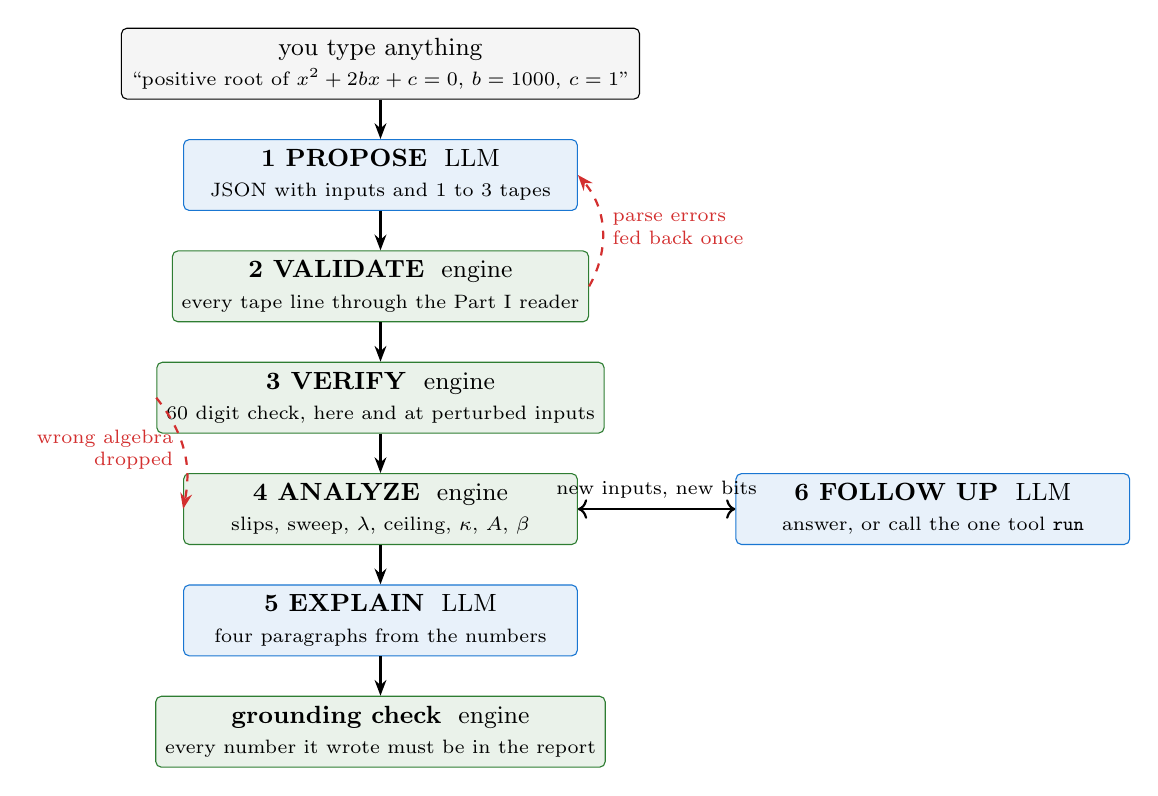
\begin{tikzpicture}[
  node distance=5mm and 12mm,
  box/.style={draw, rounded corners=2pt, align=center, minimum width=50mm, minimum height=9mm, font=\small},
  llm/.style={box, fill=askblue!10, draw=askblue},
  eng/.style={box, fill=chipgreen!10, draw=chipgreen},
  arr/.style={-{Stealth[length=2mm]}, thick},
  back/.style={-{Stealth[length=2mm]}, thick, dashed, trapred}]
\node[box, fill=gray!8] (in) {you type anything\\ \scriptsize ``positive root of $x^2+2bx+c=0$, $b=1000$, $c=1$''};
\node[llm, below=of in] (prop) {\textbf{1 PROPOSE} \ LLM\\ \scriptsize JSON with inputs and 1 to 3 tapes};
\node[eng, below=of prop] (val) {\textbf{2 VALIDATE} \ engine\\ \scriptsize every tape line through the Part I reader};
\node[eng, below=of val] (ver) {\textbf{3 VERIFY} \ engine\\ \scriptsize 60 digit check, here and at perturbed inputs};
\node[eng, below=of ver] (ana) {\textbf{4 ANALYZE} \ engine\\ \scriptsize slips, sweep, $\lambda$, ceiling, $\kappa$, $A$, $\beta$};
\node[llm, below=of ana] (exp) {\textbf{5 EXPLAIN} \ LLM\\ \scriptsize four paragraphs from the numbers};
\node[eng, below=of exp] (grd) {\textbf{grounding check} \ engine\\ \scriptsize every number it wrote must be in the report};
\node[llm, right=of ana, xshift=8mm] (ag) {\textbf{6 FOLLOW UP} \ LLM\\ \scriptsize answer, or call the one tool \texttt{run}};
\draw[arr] (in) -- (prop);
\draw[arr] (prop) -- (val);
\draw[arr] (val) -- (ver);
\draw[arr] (ver) -- (ana);
\draw[arr] (ana) -- (exp);
\draw[arr] (exp) -- (grd);
\draw[back] (val.east) to[bend right=35] node[right, font=\scriptsize, align=left] {parse errors\\ fed back once} (prop.east);
\draw[back] (ver.west) to[bend left=25] node[left, font=\scriptsize, align=right] {wrong algebra\\ dropped} (ana.west);
\draw[arr, <->] (ag) -- (ana) node[midway, above, font=\scriptsize] {new inputs, new bits};
\end{tikzpicture}
\end{center}

\subsection*{Division of labor}
\begin{center}
\begin{tabularx}{\textwidth}{@{}lX@{}}
\toprule
the LLM & reads any phrasing, LaTeX or prose, picks out the inputs, writes tape 1 exactly as the user meant it, proposes equal rewrites it is sure of, and explains the finished numbers in plain words \\
the engine & parses every tape line with the Part I reader, evaluates all tapes in 60 digits to catch wrong algebra, runs the forward pass and the backward sweep, computes every number, and checks that the explanation only quotes numbers that exist \\
neither & the LLM never adds, multiplies or rounds anything, and the engine never guesses what the user meant \\
\bottomrule
\end{tabularx}
\end{center}

\subsection*{Existing LLM ideas and where each one is used}
\begin{center}
\small
\begin{tabularx}{\textwidth}{@{}lXX@{}}
\toprule
idea & where & why it matters here \\
\midrule
program aided LMs, tool use & step 1, the model writes a tape, the interpreter runs it & arithmetic by a language model is the one thing a rounding error tool cannot afford \\
structured output, a JSON contract & every LLM reply is one JSON object with fixed keys & the engine can validate it mechanically and feed errors back \\
few shot prompting & three worked examples of the contract inside the prompt & the tape language is small and unusual, examples teach it faster than rules \\
self refine & validation problems are returned to the model once & most JSON or tape slips are fixed on the second try \\
verification by execution & step 3, all tapes compared in 60 digits at the given and at perturbed inputs & an equal looking rewrite that is wrong algebra is dropped with numeric evidence \\
grounded generation plus a faithfulness check & step 5, the narrative is checked number by number against the report & an invented number in an explanation is worse than no explanation \\
ReAct style agent with one tool & step 6, answer or call \texttt{run(inputs, bits)} and then answer & lets the student ask ``what if $b = 10^6$'' or ``single precision'' in words \\
temperature zero & every call & the same question should give the same tape \\
\bottomrule
\end{tabularx}
\end{center}

\subsection*{The contract}
\begin{lstlisting}
{"reading": "y = -b + sqrt(b^2 - c)",
 "inputs":  {"b": "1000", "c": "1"},      <- copied as strings, the engine makes them exact
 "missing": [],                           <- input names the user forgot
 "tapes": [
   {"name": "textbook",
    "lines": ["t1 = b*b", "t2 = t1 - c", "t3 = sqrt(t2)", "y = -b + t3"],
    "why": "as written"},
   {"name": "conjugate",
    "lines": ["t1 = b*b", "t2 = t1 - c", "t3 = sqrt(t2)", "t4 = b + t3", "y = -c / t4"],
    "why": "multiply top and bottom by b + sqrt(b^2 - c)"}]}
\end{lstlisting}
Three prompts, one per role. \textbf{PROPOSE} carries the tape language (the allowed operations, one rounded operation per line, last line named \texttt{y}, keep the user's order in tape 1, never do arithmetic) and the three examples. \textbf{EXPLAIN} asks for four titled paragraphs, at most three sentences each, every number copied from the report. \textbf{AGENT} allows exactly two replies, \texttt{run} with new inputs or bits, or \texttt{answer}. The mock provider in the file obeys the same three roles, so the whole pipeline and its self test run offline.

\subsection*{Guards, one per failure}
\begin{center}
\begin{tabularx}{\textwidth}{@{}lX@{}}
\toprule
failure & guard \\
\midrule
the model's rewrite is wrong algebra & step 3 evaluates every tape in 60 digits at the user's inputs and at three perturbed points, a mismatch above $10^{-30}$ relative drops the tape and prints both values \\
the model mistranscribed the user's formula & when the user text itself parses as a formula, tape 1 is checked against that formula the same way \\
the model invented a number in the explanation & the grounding check extracts every number from the narrative and looks for it (within 5 percent) in the engine report, misses are listed in red \\
a value is missing & the \texttt{missing} list, and command line \texttt{name=value} pairs override the model \\
the reply is not JSON & the first \verb|{ ... }| block is extracted, one retry with the problems listed \\
the agent keeps calling the tool & three calls at most, then the comparison table is the answer \\
no API key & \texttt{--provider mock} runs the same pipeline with a rule based stand in \\
\bottomrule
\end{tabularx}
\end{center}

\subsection*{How to run}
\begin{lstlisting}
pip install anthropic mpmath
export ANTHROPIC_API_KEY=...
python rounderr_ai.py "positive root of x^2 + 2bx + c = 0 with b = 1000, c = 1" --tex ai.tex --pdf
python rounderr_ai.py "\frac{1-\cos x}{x^2} at x = 1e-4" --lang zh
python rounderr_ai.py "Horner for 2x^3 - 3x + 1" x=1.0001 --bits 24
python rounderr_ai.py "..." --provider openai --base-url http://localhost:11434/v1 --model llama3.1
python rounderr_ai.py "..." --provider mock          # no key, same pipeline
python rounderr_ai.py --selftest
\end{lstlisting}
After the report the program waits for follow up questions. ``why is t5 to blame'' is answered from the report. ``what if b = 1e6'' or ``single precision'' makes the model call \texttt{run}, the engine reruns, and the answer comes from the new report. Everything, including the follow ups, goes into the LaTeX report.

\subsection*{What the self test checks}
A deliberately wrong rewrite is dropped by the 60 digit check. The quadratic yields two tapes, both kept, $A = 2\times10^{6}$ and $2.5$. The narrative passes the grounding check, and an invented number fails it. ``single precision'' reruns the engine at 24 bits, ``b = 1e6'' reruns with the new input. Plain formula text goes through the generic path and is verified against the user's own formula.

\subsection*{How to evaluate it for the write up}
The engine is an oracle, so grading is automatic. Take the fifteen formulas of the Part I validation table as a benchmark, each written in three styles (plain, LaTeX, prose). For each model (a small one, a large one, and the mock as a rule based baseline) measure three rates. Tape correctness, the share of tape 1 that pass verification against the user's formula. Rewrite discovery, the share of unstable cases where a proposed tape is kept and has $A$ under $\max(10,n)\max(1,\kappa)$. Grounding, the share of narratives with no loose number. Report the three rates and the median wall time per formula. That table is the AI half of the project, the Part I numbers are the numerical half.

\begin{trap}[What this layer does not change]
Every number in a report still comes from the Part I engine. If the LLM is removed, \texttt{rounderr.py} still works on its own with its rule based reader and rewrite patterns. The LLM widens what can be typed and what can be asked, it does not touch the mathematics.
\end{trap}


\clearpage
\section*{Part III \quad One machine (\texttt{rounderr\_app.py}) and Bean (\texttt{rounderr\_bean.py})}

\begin{idea}[The whole pipeline in one window]
\texttt{python rounderr\_app.py} opens a local page. Type on the left, press Analyze, read the tabs on the right. Nothing leaves the computer unless a model reader is switched on.
\[
\text{input} \to \text{READ} \to \text{TAPE} \to \text{HASH} \to \text{table lookup} \to \text{matrix SWEEP} \to \text{BEAN} \to \text{DATA}
\]
\end{idea}

\begin{center}
\begin{tabularx}{\textwidth}{@{}lX@{}}
\toprule
stage & what it does and where it lives \\
\midrule
READ & the Part I reader, or a model that writes tapes (Part II). Numbers may sit in the text, as in ``\texttt{... with b = 1000, c = 1}'' \\
TAPE & one line per rounded step, shown as a paper strip with a blame bar per line \\
HASH & SHA 256 of the tape structure. Operations and wiring only, no numbers and no names, so $ab + c$ and $pq + r$ get the same key. The engine makes it, not the model, so it is reproducible \\
table & \texttt{rounderr\_cache.json}. Per key it keeps the pattern of $L$, Bean's answer and a hit count. Model proposals are kept under a hash of the typed text, so the same text never calls the model twice \\
SWEEP & $L^{T}\lambda = w$ by back substitution. For random trials the tape is compiled once per key and every input runs at once, each $\lambda_i$ is a column of numbers (numpy) \\
BEAN & the tape is translated to a Bean program and type checked. Bean's bound holds for all inputs, the sweep holds at these inputs \\
DATA & every run is a row in the log, trials give distributions and the worst inputs found, exports are CSV, \texttt{.tex} and PDF \\
\bottomrule
\end{tabularx}
\end{center}

\subsection*{Developer tab}
The window has a Developer tab for anyone working on the code. It lists the nine stages in run order. Each stage opens to three things. What the stage is designed to do. What it received and produced on the current run (the text after each reading step, the tape, the exact string that was hashed and the table entry, every line's operands, computed value, exact value, slip and $d$, every $\lambda$ update of the sweep in order, the verdict arithmetic with the numbers filled in, the Bean program and Bean's raw output, the model's JSON when a model was used). And the source of the functions that did it, read live from the files with \texttt{inspect}, with file names and line numbers. Below that are the file map, the local API routes and the raw JSON of the run. The same trace prints in a terminal with \texttt{python rounderr\_app.py --trace "formula with x = 1"}.

\subsection*{The fast sweep}
\texttt{FastTape} walks the tape once with arrays in place of numbers. Forward gives the values, the exactness flags $d_i$ (Sterbenz, powers of two, small integers, written as array tests) and the local partials. Backward is the same six line loop, now on columns. It returns $A$, $\kappa$ and $\beta_1$ for every input. The self test checks it against the full engine on all examples (largest gap $2\times10^{-16}$). On the quadratic, 1000 inputs take about 2 milliseconds. The slow part of the full engine is the exact slips and the 60 digit reference, which the fast path skips, so the worst input found is rerun through the full engine to confirm it.

\subsection*{Bean}
Translation rules. $a+b$ and $a-b$ become \texttt{add} and \texttt{sub}. $a\cdot b$ becomes \texttt{mul}, or \texttt{dmul} when one side is reused. $a/b$ becomes \texttt{div} inside a \texttt{case}. A negation is folded into the next add or sub. A value used more than once must be discrete and may only multiply. Constants become inputs. \texttt{sqrt}, \texttt{cos} and the rest are not expressible. To compare, an output error $\Delta y$ is turned into the smallest relative change of the inputs Bean may perturb, $|\Delta y| / \sum_j |g_j x_j|$.

\begin{center}
\begin{tabular}{@{}lrrrr@{}}
\toprule
formula & Bean bound ($\varepsilon$) & adjoint ceiling ($u$) & measured ($u$) & share used \\
\midrule
sum of 4 & 3 & 1.9 & 0.25 & 13\% \\
2 by 2 determinant, nearly singular & 1.5 & 0.25 & 0.036 & 2\% \\
Horner cubic near a triple root & 6 & 0.625 & 0.1 & 3\% \\
sum of 50, worst of 200 random inputs & 49 & 12.9 & 1.78 & 7\% \\
dot product of 20, worst of 200 & 20 & 9.01 & 2 & 16\% \\
Horner degree 20, worst of 200 & 40 & 14.1 & 2.04 & 10\% \\
\bottomrule
\end{tabular}
\end{center}
Bean typed 11 of 18 test formulas. In 608 engine runs the measured backward error never left Bean's bound. Bean could not take 7 formulas (no \texttt{sqrt} or \texttt{cos}, or a reused value outside a multiply), and the engine calls 3 of those stable, so a rejection is not a proof of instability. The comparison also fixed the engine. A fixed cutoff of 10 called a 49 step sum unstable while Bean proves it stable, so the cutoff is now $\max(10, n)$.

\subsection*{Run it}
\begin{lstlisting}
pip install mpmath numpy            (anthropic too, for the Claude reader)
python rounderr_app.py              opens the window
python rounderr_app.py --bean path/to/bean.exe
python rounderr_app.py --selftest   6 checks
\end{lstlisting}
Bean is optional. Build it from \url{https://github.com/Athena-Types/Bean} with \texttt{opam install --deps-only .} and \texttt{dune build}. Without it the Bean tab still shows the translated program.

\section*{References}
\begin{itemize}
\item S. Linnainmaa, \emph{The representation of the cumulative rounding error of an algorithm as a Taylor expansion of the local rounding errors}, MS thesis, University of Helsinki, 1970.
\item S. Linnainmaa, Taylor expansion of the accumulated rounding error, \emph{BIT} 16 (1976) 146--160.
\item S. Linnainmaa, Error linearization as an effective tool for experimental analysis of the numerical stability of algorithms, \emph{BIT} 23 (1983) 346--359.
\item D. Bindel, Adjoints for roundoff sensitivity analysis, FPTalks, 6 Aug 2026, \url{https://www.cs.cornell.edu/~bindel/present/2026-08-fptalks.pdf}.
\item N. J. Higham, \emph{Accuracy and Stability of Numerical Algorithms}, 2nd ed., SIAM, 2002 (chapters 1, 3, 4, 5).
\item P. Langlois, Automatic linear correction of rounding errors (CENA), \emph{BIT} 41 (2001) 515--539.
\item A. Solovyev et al., Rigorous estimation of floating point round off errors with symbolic Taylor expansions (FPTaylor), \emph{ACM TOPLAS} 2018.
\item H. Menon et al., ADAPT, automated algorithmic differentiation for floating point precision tuning, SC 2018.
\item A. Das et al., Scalable yet rigorous floating point error analysis (SATIRE), SC 2020.
\item A. Kellison, \emph{Type based approaches to rounding error analysis}, PhD dissertation, 2025, arXiv 2501.14598 (NumFuzz and Bean, with Bindel and Hsu).
\end{itemize}
\end{document}
